\documentclass[12pt, a4paper]{article}

\usepackage[italian]{babel}
\usepackage[utf8]{inputenc}
\usepackage[T1]{fontenc}
\usepackage{graphicx}
\usepackage{subfig}
\usepackage{caption}
\usepackage{geometry}
\usepackage{color}
\usepackage{amsmath}
\usepackage{amssymb}
\usepackage{booktabs}
\usepackage{tabularx}
\usepackage{wrapfig}
\geometry{a4paper,top=1.5cm,bottom=2cm,left=1.25cm,right=1.5cm,heightrounded,bindingoffset=5mm}
\author{ Marasciulli Andrea \qquad  Lorenzetti Giacomo \qquad Browne Roberto}
\date{\today}
\frenchspacing 
\begin{document}

\begin{section}*{Calibrazione}

Abbiamo variato l'alimentazione dei vari PMT per vedere come cambia il numero di conteggi. I risultati di queste misure sono  riportati nelle tabelle seguenti e nel grafico di Figura \ref{tensio}. 
% tabelle

\begin{figure}[h]
\centering
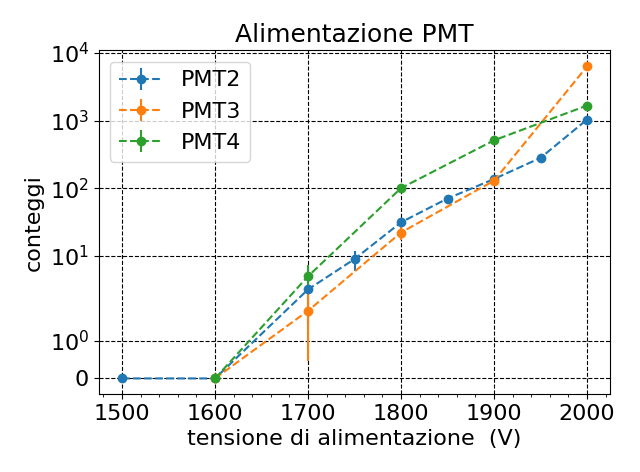
\includegraphics[width=10 cm]{tensio_pmt}
\caption{Numero di conteggi in funzione della tensione di alimentazione}
\label{tensio}
\end{figure}

Il grafico mostra chiaramente l'assenza di qualsiasi $plateau$ tranne nei punti a conteggio nullo. Abbiamo deciso di alimentare i PMT a 1800\! V perché la derivata in quel punto è minore di quella corrispondente a 1900\! V e ci sono abbastanza conteggi da permetterci una loro analisi statistica.

Dal \emph{Particle Physics Booklet 2016} sappiamo che il flusso di raggi cosmici è mediamente 180~Hz$/$\!m$^2$s. Essendo il nostro rivelatore di area $A=l_1l_2=48.0\pm0.1$\! cm $\cdot \, 40.0\pm0.1$\! cm$=1920\pm6$\! cm$^2$ ci aspettiamo il passaggio di 34.6$\pm$0.1 particelle$/$s. Questo numero è simile ai conteggi ottenuti a 1800\! V con soglia V$_{thr}\simeq-376$\! mV. 

\end{section}


\begin{section}*{Modulo di coincidenze}

Per effettuare il conteggio delle coincidenze abbiamo collegato le uscite dei discriminatori al modulo di coincidenze FE260 e la sua uscita al canale 5 dello scaler. I canali 1 e 2 di quest'ultimo sono collegati al PMT4 e al PMT2 attraverso il discriminatore. Le soglie di entrambi sono massime, ovvero -0.410\! V misurate dal testpoint.

\end{section}

\end{document}